\section{The Proposed Beamlet Propagation algorithm}
\label{sec:algorithm}
The transfer matrix method of GBD is \added{the preferred algorithm to develop} because of the recent developments by Worku and Gross to include modified GBD\cite{Worku19}. \added{However, because the implementation is not public we must derive the full algorithm using the concepts described in \hyperref[sec:methods]{Section \ref{sec:methods}}}. \added{The basic concept of propagating a single beamlet through an arbitrary optical system is illustrated in Figure \ref{fig:gaussian_prop_diagram}. A Gaussian beam is placed at some position $\mathbf{r}_{cen,S}$ in the source plane where the initial decomposition occurs. The central ray (shown in black on Figure \ref{fig:gaussian_prop_diagram}) that tracks the position of the Gaussian beam and the differential rays (shown in light red and blue on Figure \ref{fig:gaussian_prop_diagram}) that define the propagation are traced to the evaluation plane using a ray tracing engine. The central ray position ($\mathbf{r}_{cen,E}$), and direction ($\mathbf{k}_{cen,E}$) on the evaluation plane are used to define the transversal plane which includes the point where we wish to evaluate the Gaussian field. The differential rays and the central ray are transformed to the transversal plane in order to compute the ABCD matrix that describes the propagation of the Gaussian beam from the source plane to the transversal plane. We use this matrix to compute the influence of this beam on the field evaluation point.} \added{Every beamlet used in the initial field decomposition is propagated to each point on the evaluation plane this way, and the coherent superposition of the beamlets at the evaluation plane represents the propagated field.}

\begin{figure}[H]
    \centering
    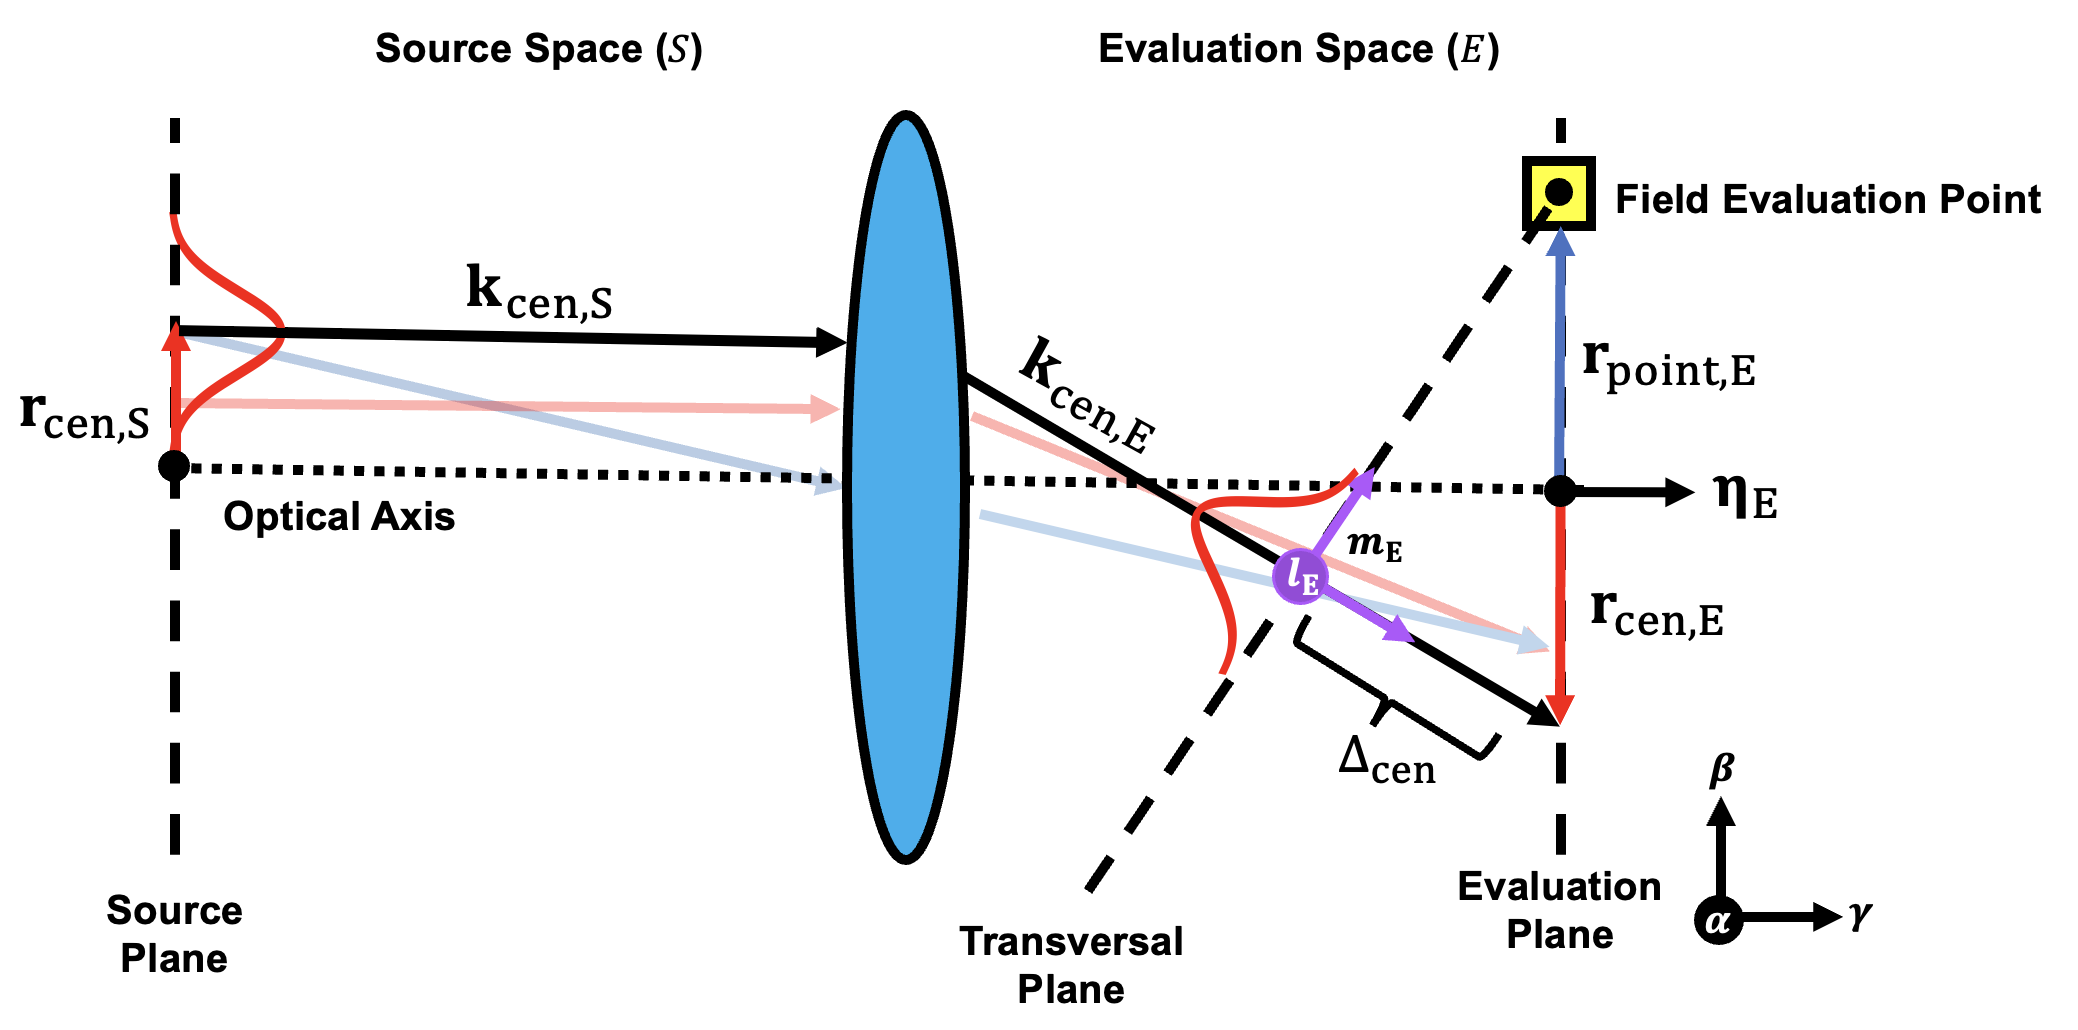
\includegraphics[width=\textwidth]{gbd_prop_diagram.png}
    \caption{\added{Diagram illustrating the geometry of GBD and the relevant data used in the propagation calculation for a single beamlet (shown in red). GBD begins by tracing the central ray (black) and differential rays (light red and blue) from the source plane (left) to the evaluation plane (right). The rays must be propagated from the evaluation plane to the transversal plane, which is normal to the central ray and intersects a point at which the field is evaluated (yellow box). The difference of the differential ray data with the central ray data on the transversal plane gives us the ABCD matrix used to propagate a Gaussian beamlet. We evaluate the Gaussian beamlet at the intersection of the transversal plane with the evaluation plane to get the beamlet's contribution to the total field at that point. This process is repeated for each point and each beamlet. The coherent superposition of the beamlets at the field evaluation points yields the final propagated field.}}
    \label{fig:gaussian_prop_diagram}
\end{figure}

\added{In this section we derive the formula to compute the propagation of a ray to the transversal plane, and how to use this data to compute the ABCD matrix and the contribution of a Gaussian beamlet to a point on the evaluation plane using the methods described in Section \ref{sec:methods}.} \added{We refer to several vectors in the algorithm below that are expressed using the convention $\mathbf{u}_{v,W}$. $\mathbf{u}$ is the data type of the vector, typically $\mathbf{r}$ if a position or $\mathbf{k}$ if a direction. $v$ denotes what item the vector belongs to, "cen" means it belongs to the central ray and "point" means a point on the evaluation plane. $W$ refers to the coordinate system of the vector, $S$ for "source space",} \added{$E$ for "evaluation space"}, \added{or $T$ for "transversal plane". The relevant parameters used in the propagation algorithm are shown in Figure \ref{fig:gaussian_prop_diagram}, and are referenced throughout the procedure below.}

\subsection{Propagating rays to the transversal plane}
\added{A GBD simulation begins by running a ray trace though an optical system in the user's preferred design code. GBD needs the ray data at the plane where the decomposition occurred (the source plane) and the plane where we choose to observe the field (the evaluation plane). We use the ray data in evaluation space to propagate the rays to the transversal plane, where Equation \ref{eq:gaussian_prop} valid.}

\added{We first need to derive the propagation distance $\Delta_{ray}$ for the central and four differential rays. To do so, we find the intersection of the line defined by the ray we want to propagate $\mathbf{k}_{ray,E}$ and the plane normal to the central ray of the Gaussian beam $\mathbf{k}_{cen,E}$ which intersects the evaluation point $\mathbf{r}_{point,E}$. This plane is the transversal plane, and is defined by Equation \ref{eq:plane}}

\begin{equation}
    \added{\mathbf{k}_{cen,E} \cdot (\mathbf{r} - \mathbf{r}_{point,E}) = 0.}
    \label{eq:plane}
\end{equation}

\added{The line along the ray is defined by Equation \ref{eq:line}}

\begin{equation}
    \added{\mathbf{r} = \mathbf{r}_{ray,E} + \mathbf{k}_{ray,E}\Delta_{ray},}
    \label{eq:line}
\end{equation}

\added{where $\cdot$ denotes the dot product and $\mathbf{r}$ is the space of all points that satisfy Equations \ref{eq:plane} and \ref{eq:line}. To find the distance a ray needs to propagate along its own path in free space to intersect the transversal plane, we substitute $\mathbf{r}$ in Equation \ref{eq:plane} for Equation \ref{eq:line} and solve for $\Delta_{ray}$. The result is given by Equation \ref{eq:delta}}


\begin{equation}
    \added{\Delta_{ray} = - \frac{\mathbf{k}_{cen,E} \cdot (\mathbf{r}_{ray,E} - \mathbf{r}_{point,E})}{\mathbf{k}_{cen,E} \cdot \mathbf{k}_{ray,E}}}.
    \label{eq:delta}
\end{equation}

\added{The expression in Equation \ref{eq:delta} is written for the general case of propagating a ray from the evaluation plane to the transversal plane. It is applied to the central and differential rays by substituting $\mathbf{r}_{ray,E}$ and $\mathbf{k}_{ray,E}$ for the position and direction associated with the ray to propagate. We update the ray positons by invoking Equation \ref{eq:line}. The ray position on the transversal plane ($\mathbf{r}'_{ray,E}$) is given in Equation \ref{eq:prop_ray}}

\begin{equation}
    \added{\mathbf{r}'_{ray,E} = \mathbf{r}_{ray,E} + \mathbf{k}_{ray,E}\Delta_{ray}.}
    \label{eq:prop_ray}
\end{equation}

\added{However, these coordinates are still expressed in the basis of the evaluation plane. We must next rotate the ray coordinates into the transversal plane coordinate system so that they are orthogonal to the propagation direction.}

\subsection{Transformation to the transversal plane}
\added{In the evaluation plane coordinate system, we define the orthogonal basis vectors $\boldsymbol{{\alpha}}$,$\boldsymbol{{\beta}}$,and $\boldsymbol{{\gamma}}$ (shown in black on Figure \ref{fig:gaussian_prop_diagram} to the right of the evaluation plane), to be the directions along the $x$,$y$, and $z$ axes respectively.} \added{Similarly, the transversal plane is defined by basis vectors $\mathbf{l}_{E}$,$\mathbf{m}_{E}$,$\mathbf{k}_{cen,E}$, (shown in purple on Figure \ref{fig:gaussian_prop_diagram}) which are the analogous $x$,$y$, and $z$ directions for the transversal plane. To compute these directions, we start by taking the cross product of the central ray $\mathbf{k}_{cen,E}$ with the surface normal of the evaluation plane $\boldsymbol{\eta_{E}}$ (shown in black on the right of Figure \ref{fig:gaussian_prop_diagram})}

\begin{equation}
    \added{\mathbf{l}_{E} = \mathbf{k}_{cen,E} \times \mathbf{\eta_{E}}.}
    \label{eq:compute_lbasis}
\end{equation}

\added{A feature of Equation \ref{eq:compute_lbasis} is that the $\mathbf{l}_{E}$ is orthogonal to both the central ray and the surface normal. Similarly, to determine our final basis vector which is mutually orthogonal to both the central ray and $\mathbf{l}_{E}$ basis vector we compute their cross product}

\begin{equation}
    \added{\mathbf{m}_{E} = \mathbf{k}_{cen,E} \times \mathbf{l}_{E}.}
    \label{eq:compute_mbasis}
\end{equation}

\added{These vectors form a complete basis that describe the coordinate system of the transversal plane, but are expressed in the coordinate system of the evaluation plane. Therefore, we can construct an orthogonal transformation matrix that performs a rotation of basis from the evaluation plane to the transversal plane. This matrix is shown in Equation \ref{eq:orthomatrix}}

\begin{equation}
\centering
\added{\mathbf{O} = }
\added{
    \begin{pmatrix}
     l_{\alpha} & l_{\beta} & l_{\gamma} \\
     m_{\alpha} & m_{\beta} & m_{\gamma} \\
     k_{\alpha} & k_{\beta} & k_{\gamma} \\
    \end{pmatrix},}
    \label{eq:orthomatrix}
\end{equation}

\added{Where $\mathbf{l}_{E}$,$\mathbf{m}_{E}$, and $\mathbf{k}_{cen,E}$, are written as $l,m,k$ respectively for brevity and are shown in Equation \ref{eq:orthomatrix} as their components projected onto the vectors $\boldsymbol{\alpha},\boldsymbol{\beta}$, and $\boldsymbol{\gamma}$. The matrix $\mathbf{O}$ is the tool we need to express our ray coordinates in terms of the transversal plane basis. This is done by a simple multiplication of the ray position and direction vectors ($\mathbf{r}'_{ray,E}$,$\mathbf{k}_{ray,E}$) with the matrix, shown in Equations \ref{eq:posbasis} and \ref{eq:dirbasis}}

\begin{equation}
    \added{\mathbf{r}_{ray,T} = \mathbf{O}\mathbf{r}'_{ray,E},}
    \label{eq:posbasis}
\end{equation}

\begin{equation}
    \added{\mathbf{k}_{ray,T} = \mathbf{O}\mathbf{k}_{ray,E}.}
    \label{eq:dirbasis}
\end{equation}

\added{The same must also be done for the field evaluation point of interest $\mathbf{r}_{point,E}$ to evaluate the Gaussian field later, shown in Equation \ref{eq:pixbasis},}

\begin{equation}
    \added{\mathbf{r}_{point,T} = \mathbf{O}\mathbf{r}_{point,E}.}
    \label{eq:pixbasis}
\end{equation}.

\added{Now that the ray data is expressed in the transversal plane coordinate system, we can use them to compute the differential ray transfer matrix used to propagate the Gaussian beamlet. }

\subsection{Computing the differential ray transfer matrix}
\added{To compute the differential ray transfer matrix for a Gaussian beam we require the five ray coordinates and directions derived in the previous subsection ($\mathbf{r}_{ray,T}$, and $\mathbf{k}_{ray,T}$), as well as the data for the same rays on the source plane ($\mathbf{r}_{ray,S}$, and $\mathbf{k}_{ray,S}$). The differential ray transfer matrix is calculated using the methods discussed in \hyperref[sec:methods]{Section \ref{sec:methods}}. Recall that an element of the ray transfer matrix is given by the difference of the central and differential ray coordinates at the source and evaluation plane (see Equation \ref{eq:Ayy}). The resultant matrix is given by Equation \ref{eq:diffmat}.} \added{The full matrix including the ray data used to compute each of the elements of Equation \ref{eq:diffmat}, can be found in \hyperref[sec:appendixA]{Appendix A}.}

\begin{center}
\begin{equation}
    \begin{pmatrix}[c | c]
        \added{\mathbf{A}} & \added{\mathbf{B}} \\
        \hline
        \added{\mathbf{C}} & \added{\mathbf{D}} \\
    \end{pmatrix} 
    =
    \begin{pmatrix}[c c | c c ]
    \added{\frac{\partial x_T}{\partial x_S}} & \added{\frac{\partial x_T}{\partial y_S}} & \added{\frac{\partial x_T}{\partial l_S}} & \added{\frac{\partial x_T}{\partial m_S}}  \\
    \added{\frac{\partial y_T}{\partial x_S}} & \added{\frac{\partial y_T}{\partial y_S}} & \added{\frac{\partial y_T}{\partial l_S}} & \added{\frac{\partial y_T}{\partial m_S}}  \\
    \hline 
    \added{\frac{\partial l_T}{\partial x_S}} & \added{\frac{\partial l_T}{\partial y_S}} & \added{\frac{\partial l_T}{\partial l_S}} & \added{\frac{\partial l_T}{\partial m_S}} \\
    \added{\frac{\partial m_T}{\partial x_S}} & \added{\frac{\partial m_T}{\partial y_S}} & \added{\frac{\partial m_T}{\partial l_S}} & \added{\frac{\partial m_T}{\partial m_S}} \\
    \end{pmatrix}
    %$
    \label{eq:diffmat}
\end{equation}
\end{center}

\added{The total ray transfer matrix can be organized into a tensor composed of 2x2 sub-matrices shown on the left hand side of Equation \ref{eq:diffmat}. These are exactly the non-orthogonal representations of the ray transfer matrix discussed in \hyperref[sec:methods]{Section \ref{sec:methods}} that we need to compute the propagated Gaussian field profile.}

\subsection{Computing the Gaussian field}
\added{The central ray serves as the coordinate origin for our Gaussian field evaluation on the transversal plane. With the position vectors effectively transformed in Equations \ref{eq:posbasis} and \ref{eq:pixbasis}, we can define our centered radial coordinate $\mathbf{r}_{o}$ as the simple difference of these two positions to center the coordinate system in Equation \ref{eq:radial_cord}}
\begin{equation}
    \added{\mathbf{r}_{o} = \mathbf{r}_{point,T} - \mathbf{r}_{cen,T}.}
    \label{eq:radial_cord}
\end{equation}
\added{Finally, we can call upon Equation \ref{eq:gaussian_prop} to perform the Gaussian field evaluation, with some added phase factors to account for the free-space propagation of the Gaussian beamlet. The result is shown in Equation \ref{eq:final_gauss}}
\begin{equation}
    \added{U(\mathbf{r}_{o}) = \frac{U_{o}}{\sqrt{det|\mathbf{A} + \mathbf{BQ_{1}^{-1}}|}} exp[\frac{-ik}{2} \mathbf{r}^{T}_{o} \mathbf{Q_{2}^{-1}} \mathbf{r}_{o} + ik\Delta_{cen} + ik\Phi_{opd}]},
    \label{eq:final_gauss}
\end{equation}

\added{where $\mathbf{Q_{2}^{-1}}$ is the propagated complex curvature matrix given by Equation \ref{eq:prop_complex}, $\mathbf{r}_{o}^{T}$ is the transpose of the coordinate from Equation \ref{eq:radial_cord}, $\Delta_{cen}$ is the propagated distance of the central ray to the transversal plane, and $\Phi_{opd}$ is the optical path experienced by the central ray through the optical system, which we get from the ray tracing engine used. Note that while the phase factors  $\Delta_{cen}$ and $\Phi_{opd}$ are not present in Equation \ref{eq:gaussian_prop}, they are necessary for GBD to correctly interfere all of the Gaussian beams that are propagated.}

The procedure outlined above is repeated for each beamlet and \added{location on the evaluation plane}. From a computational perspective this procedure is somewhat daunting. Repeating this process means the computation complexity scales \added{by the number of beamlets and number of points on the evaluation plane}, which can quickly become prohibitive. Fortunately, the algorithm described is entirely vector and matrix operations so it is simple to take advantage of broadcasted array operations in Python to vectorize the computation, and parallel computing to accelerate it. In our implementation, the vector operations described above are broadcasted such that the field of a single beamlet at all \added{points} is computed simultaneously. This operation exists in a loop over the number of beamlets. For \added{our} preliminary efforts in computational acceleration, see \hyperref[sec:appendixB]{Appendix B}.

 Note the subtlety that the propagation procedure does not depend on the elementary field of choice until the electric field is evaluated. The assumption of this propagation method is that the elementary field is paraxial about the area encompassed by the differential rays. In principle, as long as a field's propagation formula is known analytically via the general Collins integral it can be propagated with this method. Thus, GBD is a \emph{special case} of the method described \added{in this section}. Because of the history of modeling resonators with ray transfer matrices, we know the ABCD propagation laws for Laguerre-Gaussian\cite{Mei_2005} and Hermite-Gaussian\cite{CAI2002139} beams, which form complete sets. This indicates that the beamlet decomposition method would be of higher accuracy when decomposing the field into modes of higher spatial order. The formula for flattened elliptical Gaussian beams is also known\cite{CAI2002139}, which are capable of mitigating the soft-edge effect imposed by the traditional beamlet decomposition\cite{greynolds_ten_2020}. This method also works with Worku and Gross's half- and quarter-truncated Gaussian beamlets\cite{Worku19}. \added{The algorithm described in this Section is one of the key results of this study, because it can propagate the field of any known solution to the Collins integral to an arbitrary array of points. We build this algorithm into Poke to test its ability to mimic diffraction simulations with known results, and perform a comparison against commercial software.}

